
%% bare_jrnl_transmag.tex
%% V1.4
%% 2012/12/27
%% by Michael Shell
%% see http://www.michaelshell.org/
%% for current contact information.
%%
%% This is a skeleton file demonstrating the use of IEEEtran.cls
%% (requires IEEEtran.cls version 1.8 or later) with an IEEE 
%% Transactions on Magnetics journal paper.
%%
%% Support sites:
%% http://www.michaelshell.org/tex/ieeetran/
%% http://www.ctan.org/tex-archive/macros/latex/contrib/IEEEtran/
%% and
%% http://www.ieee.org/

\documentclass[journal,transmag]{IEEEtran}
\usepackage[cmex10]{amsmath}
\usepackage[]{amsfonts,amssymb}
\usepackage{algorithm2e}
\usepackage{array}
\usepackage[pdftex]{graphicx}
\usepackage{breqn}

\newcommand{\bvar}[2]{\mathbf{#1}_{#2}}
\newcommand{\stateest}[1][k]{p(\mathbf{x}_{#1} \mid \mathbf{z}_{1...#1},\mathbf{u}_{1...#1})}
\newcommand{\meas}[1][k]{p(\mathbf{z}_{#1} \mid \mathbf{x}_{#1})}
\newcommand{\motion}[1][k]{p(\mathbf{x}_{#1} \mid \mathbf{x}_{#1-1},\mathbf{u}_{#1})}
\newcommand{\imcoords}{(x_{\text{im}},y_{\text{im}})}
\newcommand{\usorientation}[1][k]{R^{\text{ us}}_{#1}}
\newcommand{\uspos}[1][k]{\vec{p}^{\text{ us}}_{#1}}
\newcommand{\shaftcoords}{[x_{\text{shaft}}, y_{\text{shaft}}]^\top}
\newcommand{\unistate}[2]{\mathbf{#1}^{\text{tip}}_{#2}}

\begin{document}
%
% paper title
% can use linebreaks \\ within to get better formatting as desired
% Do not put math or special symbols in the title.
\title{State Estimation of Steerable Needles Using Tracked 2D Doppler Ultrasound}


% author names and affiliations
% transmag papers use the long conference author name format.

\author{\IEEEauthorblockN{Joseph D. Greer\IEEEauthorrefmark{1},
Troy K. Adebar\IEEEauthorrefmark{1},
Allison M. Okamura\IEEEauthorrefmark{1}, 
\IEEEauthorblockA{\IEEEauthorrefmark{1}Deparment of Mechanical Engineering,
Stanford University, Stanford, CA 94305 USA}
\thanks{Manuscript received December 1, 2012; revised December 27, 2012. 
Corresponding author: M. Shell (email: http://www.michaelshell.org/contact.html).}}
}

% The paper headers
\markboth{Journal of \LaTeX\ Class Files,~Vol.~11, No.~4, December~2012}%
{Shell \MakeLowercase{\textit{et al.}}: Bare Demo of IEEEtran.cls for Journals}
% The only time the second header will appear is for the odd numbered pages
% after the title page when using the twoside option.
% 
% *** Note that you probably will NOT want to include the author's ***
% *** name in the headers of peer review papers.                   ***
% You can use \ifCLASSOPTIONpeerreview for conditional compilation here if
% you desire.

% for Transactions on Magnetics papers, we must declare the abstract and
% index terms PRIOR to the title within the \IEEEtitleabstractindextext
% IEEEtran command as these need to go into the title area created by
% \maketitle.
% As a general rule, do not put math, special symbols or citations
% in the abstract or keywords.
\IEEEtitleabstractindextext{%
\begin{abstract}
The abstract goes here.
\end{abstract}

% Note that keywords are not normally used for peerreview papers.
\begin{IEEEkeywords}
IEEEtran, journal, \LaTeX, magnetics, paper, template.
\end{IEEEkeywords}}



% make the title area
\maketitle


% To allow for easy dual compilation without having to reenter the
% abstract/keywords data, the \IEEEtitleabstractindextext text will
% not be used in maketitle, but will appear (i.e., to be "transported")
% here as \IEEEdisplaynontitleabstractindextext when the compsoc 
% or transmag modes are not selected <OR> if conference mode is selected 
% - because all conference papers position the abstract like regular
% papers do.
\IEEEdisplaynontitleabstractindextext
% \IEEEdisplaynontitleabstractindextext has no effect when using
% compsoc or transmag under a non-conference mode.




% For peer review papers, you can put extra information on the cover
% page as needed:
% \ifCLASSOPTIONpeerreview
% \begin{center} \bfseries EDICS Category: 3-BBND \end{center}
% \fi
%
% For peerreview papers, this IEEEtran command inserts a page break and
% creates the second title. It will be ignored for other modes.
\IEEEpeerreviewmaketitle



\section{Introduction}
\IEEEPARstart{R}{obotic} needle steering enables the controlled insertion of highly flexible needles along planned, 3D paths through the body to an anatomical target. Percutaneous interventions, such as tumor ablation and biopsy may benefit from robotic needle steering due to several key benefits afforded by needle steering. Robotic control of  needle insertion promises higher needle tip placement accuracy, and enables active correction of unexpected deflections of the needle away from its desired trajectory as the needle is inserted. The flexible nature of steerable needles allows the needle to be steered around sensitive anatomy such as vasculature, as well as providing greater freedom of choice over needle insertions sites when targeting a specific location in the body compared to rigid needles currently used in percutaneous procedures. Finally, the ability to target multiple locations through a single puncture is particularly advantageous in our target application, radiofrequency ablation of tumors in the liver.

\section{Static Needle Segmentation}
Repeat MICCAI paper.

\section{Probabilistic State Estimation}
\begin{figure}[!t]
\centering
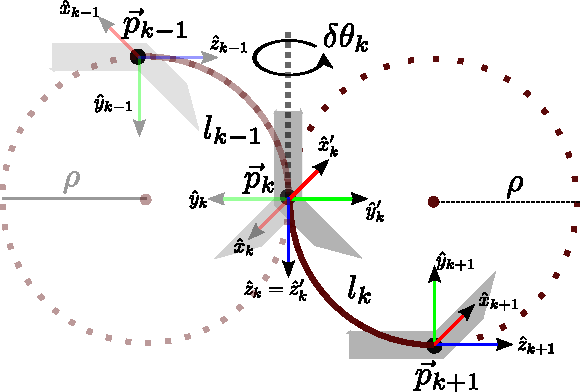
\includegraphics[scale=0.9]{Figures/NeedleKinematics.pdf}
\caption{Needle Kinematics}
\label{fig_nk}
\end{figure}

In this work, the state estimation problem for steerable needles is formulated in the Bayesian Filtering framework \cite{Thrun:2005}.
\begin{align}  \label{eqn:stateest}
&\underbrace{\stateest}_{\text{current state estimate}} = \eta \underbrace{\motion}_{\text{motion model}} \underbrace{\meas}_{\text{measurement model}}
\end{align}
The left side of equation (\ref{eqn:stateest}) is a probability distribution representing the needle's state, $\bvar{x}{k}$.  With certain independence assumptions for the needle's states and measurements \cite{Thrun:2005}, this probability distribution can be decomposed into two distributions. Each distribution can be computed in an efficient manner:  the motion model predicts how the system will respond to input $\bvar{u}{k}$, and the measurement model captures the distribution of measurements one would expect given the system's state.   In practice, we approximate the Bayesian filtering method using a particle filter \cite{Gordon1993}.


\subsection{Needle Steering State} \label{subsec:state}
Figure \ref{fig_nk} provides a diagram of the unicycle kinematic model for needle steering.  In this model, the state of the system $\bvar{x}{k} =  \left[\vec{p}_k, R_k\right]^\top$ is completely defined by the position of the needle tip, $\vec{p}_k$ and the orientation of a frame attached to the needle tip, $R_k = \left[\hat{x}_k,\hat{y}_k,\hat{z}_k\right] \in \text{SO(3)}$.  For state estimation, we augment the unicycle kinematic state with the ultrasound transducer position and orientation, $\usorientation$ and $\uspos$.  This information is provided by an electromagnetic tracker which is fixed to the ultrasound transducer.  Finally,  we also augment the unicycle kinematic model state with the $N$ most recent command inputs $\bvar{u}{k-1...k-N}$.  This makes it possible to estimate the shaft's position and orientation, which is important for the measurement model described in section \ref{subsec:measurement} below.
\begin{dmath*}
\bvar{x}{k} =  \left[\underbrace{\vec{p}_k,}_{\text{tip pos.}} \underbrace{R_k,}_{\text{tip orientation}} \underbrace{\uspos,}_{\text{transducer pos.}} \underbrace{\usorientation,}_{\text{transducer orientation}} \underbrace{\bvar{u}{k-1,...,k-N}}_{\text{previous commands}}\right]^\top
\end{dmath*}


\subsection{Motion Model} \label{subsec:unicycle}
In this work, we use the unicycle kinematic model proposed in \cite{Park2005}.  This model has previously been used and validated for closed loop control of steerable needles in \cite{Majewicz2013} and \cite{adebar2014recursive}.  In the unicycle kinematic model, steerable needles are assumed to naturally follow circular paths of constant curvature in a plane determined by the orientation and position of the needle's tip.  Control of the needle is achieved through two degrees of freedom, insertion and rotation of the needle about its axis.

Using the unicycle kinematic model for needle steering, a state transition function can be defined for the propagation of the needle tip position and orientation over time in response to control inputs and disturbances
\begin{equation*}
\unistate{x}{k+1} = f_{\text{uni}}(\unistate{x}{k}, \bvar{u}{k}, \bvar{w}{k})
\end{equation*}  
where $\unistate{x}{k+1}$ is the needle tip's state at time-step $k+1$. $\bvar{u}{k}$ and $\bvar{w}{k}$ are the control and disturbance vectors at time $k$ and are described below.  

At each time-step, the needle is rotated about its axis by $\delta \theta_k$ and inserted a distance $l_k$.  These actions define the control input 
\begin{equation*}
\bvar{u}{k} = \left[l_k, \delta\theta_k\right]^\top
\end{equation*}  

During an insertion, the unicycle kinematic model assumes the needle will travel along a circular arc.  The radius of curvature of this arc, $\rho$, is assumed to be constant and is governed by the stiffness of both the tissue and needle.  

A state update is first calculated assuming no process noise, producing a new ideal state, $\unistate{x}{\text{ideal}} = \left[\vec{p}_{\text{ ideal}}, R_{\text{ ideal}}\right]$.  This is done by rotating the coordinate frame attached to the needle tip, $R_k$, about $\hat{z}_k$ by $\delta \theta$ radians to yield an intermediate frame $R' = [\hat{x}', \hat{y}', \hat{z}']$:
\begin{equation*}
R' = R_{\hat{z}_k}(\delta\theta)R_k
\end{equation*}
In the plane defined by intermediate tip frame axes $\hat{y}'_k$ and $\hat{z}'_k$, the tip position is moved along a $\frac{l_k}{\rho}$ radian arc segment of length $l_k$ to yield a new tip position, $\vec{p}_{\text{ideal}}$.  Finally, $R'$ is rotated by $\frac{l_k}{\rho}$ radians about $\hat{x}'$ to yield an updated coordinate frame
\begin{equation*}
R_{\text{ideal}} = [\hat{x}_{\text{ideal}}, \hat{y}_{\text{ideal}}, \hat{z}_{\text{ideal}}] = R_{\hat{x}'_k}\left(\frac{l_k}{\rho}\right)R'
\end{equation*}
so that $\hat{z}_{\text{ideal}}$ is tangent with the needle's trajectory at time $k+1$.  

The ideal needle state update described above has error from both inaccuracies in the kinematic model as well as disturbances such as tissue in-homogeneity, vasculature, and tissue fascia.  Because of this, the ideal unicycle kinematic model was modified in \cite{adebar2014recursive} to account for error in both position and orientation.  These errors are captured in the process noise random variable 
\begin{equation*}
\bvar{w}{k} = \left[\vec{w}_{p_k}, W_{k}\right]
\end{equation*}  
which has a position noise component, $\vec{w}_{p_k}$ and an orientation noise component, $W_{k}$.  $\vec{w}_{p_k}$ is added to $\vec{p}_{\text{ideal}}$ to yield the final position $\vec{p}_{k+1}$.
Similarly, the orientation noise component perturbs $R_{ideal}$ to yield the final orientation $R_{k+1}$
\begin{align*}
\vec{p}_{k+1} &= \vec{p}_{\text{ideal}}+\vec{w}_{p_k} \\
R_{k+1} &= W_{k}R_{\text{ideal}}
\end{align*}
Finally, we define the full state transition function, $f$, in terms of $f_{\text{uni}}$ as 
\renewcommand*{\arraystretch}{1.2}
\begin{equation*}
\bvar{x}{k+1} = \begin{bmatrix} \vec{p}_{k+1} \\ 
								R_{k+1} 	  \\ 
								\uspos[k+1] \\ 
								\usorientation[k+1] \\
								\bvar{u}{k,...,k-N+1}
				\end{bmatrix}
				=
				\begin{bmatrix}
				f_{\text{uni}}\left(\begin{bmatrix} \vec{p}_k \\ R_k \end{bmatrix}, \bvar{w}{k}, \bvar{u}{k} \right) \\
				\uspos[k+1] \\
				\usorientation[k+1]		\\
				(\bvar{u}{k-1,...,k-N} \cup \bvar{u}{k}) \setminus \bvar{u}{k-N}
				\end{bmatrix}								
\end{equation*}
which simply updates the command history with the latest command and adds the transducer pose to the state.  Note that $\uspos, \usorientation$ and $\bvar{u}{k-1,...,k-N}$ are not treated as stochastic quantities to be estimated since they are nuisance parameters in the sense that they are not needed for control, only measurement.  In theory, a more accurate estimate of needle tip position and orientation could be achieved by treating these variables as stochastic quantities, but this would increase the dimensionality of the state space, and hence the number of particles needed, which ultimately means extra computational expense.

With the stochastic state update function, $f$, an estimate of the probability of being in state $\bvar{x}{k}$ can be calculated analytically given a previous state, action, and disturbance.  In practice, the motion model is used to generate a Monte-Carlo estimate of $p(\bvar{x}{k} \mid  \bvar{z}{k-1,...,1}, \bvar{u}{k-1,...,1})$, which amounts to repeatedly sampling previous states and disturbances, $\bvar{x}{k-1}, \bvar{w}{k-1}$, and computing $f(\bvar{x}{k-1}, \bvar{u}{k-1}, \bvar{w}{k-1})$.  
\subsection{Measurement Model} \label{subsec:measurement}
\begin{figure}[]
\centering
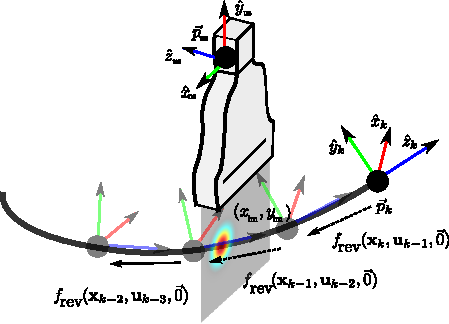
\includegraphics[scale=1]{Figures/NeedleMeasurements.pdf}
\caption{Needle Measurement Model}
\label{fig_mm}
\end{figure}
It is assumed that the ultrasound transducer is positioned so that ultrasound image plane is near the needle tip, but not on it.  In other words, the needle tip is not directly observed.  Nevertheless, by using the unicycle kinematic model and command history, hypothesis needle tip states can be propagated backward in time to shaft positions.  Because of this, measurements of the needle shaft indirectly provide information about the needle tip.

In this work, a combination of Doppler and B-mode images from a tracked 2D transducer are used for sensing the steerable needle.  As described in section \ref{sec:imageproc}, each image is processed to produce a measurement
\begin{dmath*}
\bvar{z}{k} = \left[\underbrace{x_{\text{im}},y_{\text{im}},}_{\text{image coords.}} \underbrace{d}_{\text{Doppler response}}\right]^\top
\end{dmath*}
Figure \ref{fig_mm} illustrates the components of a measurement, $\bvar{z}{k}$.  $\imcoords$ represents the estimated intersection of the needle shaft and ultrasound plane in image coordinates of the ultrasound image plane at time $k$ and $d$ is the Doppler response corresponding to the intersection.

The measurement model can be explicitly written as $\meas = p(x_{\text{im}}, y_{\text{im}}, d \mid \bvar{x}{k})$.  It is assumed that the probability of a Doppler response is independent of shaft measurement location, so that the measurement model can be decomposed into a Doppler probability and image location probability, which are calculated separately. 
\begin{align*}
p(x_{\text{im}}, y_{\text{im}}, d \mid \bvar{x}{k}) = p(d \mid \bvar{x}{k}) p(x_{\text{im}}, y_{\text{im}} \mid \bvar{x}{k})
\end{align*}

The image location probability provides information about the needle tip's orientation, lateral position, and radius of curvature.  Let $[x_{\text{shaft}}, y_{\text{shaft}}]^\top$ be the coordinates that locate the point of intersection between the needle shaft and image plane in image coordinates of the ultrasound frame at time $k$.  Given $\bvar{x}{k}$, $[x_{\text{shaft}}, y_{\text{shaft}}]^\top$ can be calculated by first propagating the needle tip and orientation, $\vec{p}_k, R_k$, backward through the unicycle kinematic model until the shaft segment between two time-steps intersects the image plane. This is done using command history $\bvar{u}{k-1,...,k-N}$.  See figure \ref{fig_mm}.  Note that backward propagation of tip state be defined in terms of $f_{\text{uni}}$ as follows
\begin{equation*}
\unistate{x}{k-1} = f_{\text{rev}}(\unistate{x}{k}, \bvar{u}{k}) = f_{\text{uni}}\left(\begin{bmatrix}\vec{p}_k \\ R_{\hat{x}}(\pi) R_k \end{bmatrix}, \bvar{u}{k}, \vec{0}\right)
\end{equation*}
It is assumed the location measurement $\left[x_{\text{im}}, y_{\text{im}}\right]^\top = [x_{\text{shaft}}, y_{\text{shaft}}]^\top + \vec{w}_{\text{im}}$ where $\vec{w}_{\text{im}} \sim \mathcal{N}(\vec{0}, \sigma_{\text{im}}^2 I)$, which means the image location probability can be calculated as  
\begin{align*}
& p(x_{\text{im}},y_{\text{im}} \mid \bvar{x}{k}) = \\
&\frac{1}{\sigma_{\text{im}} \sqrt{2 \pi}} \exp \left(\frac{\sigma_{\text{im}}^2}{2} \begin{bmatrix}x_{\text{shaft}}-x_{\text{im}} \\ y_{\text{shaft}}-y_{\text{im}} \end{bmatrix}^\top \begin{bmatrix}x_{\text{shaft}}-x_{\text{im}} \\ y_{\text{shaft}}-y_{\text{im}} \end{bmatrix} \right)
\end{align*} 

The Doppler probability, on the other hand indicates whether or not the ultrasound image plane intersects the needle shaft and hence indirectly provides information about the axial position of the needle tip.  Because Doppler response is not a perfect indicator of whether or not the ultrasound image plane intersects the needle shaft, we treat it as a probabilistic quantity.  This is done by training two distributions beforehand, $p(d \mid C)$ and $p(d \mid \neg C)$.  These distributions represent the probability of a particular Doppler response, $d$, assuming the ultrasound image plane intersects and does not intersect the needle shaft respectively.  Finally, we calculate the Doppler probability as 
\begin{equation*}
p(d \mid \bvar{x}{k}) = \left\{ \begin{array}{lr} p(d \mid C) : & \text{transducer over shaft} \\ p(d \mid \neg C) : &\text{transducer not over shaft} \end{array} \right.
\end{equation*}
\section{Conclusion}
The conclusion goes here.


% use section* for acknowledgement
\section*{Acknowledgment}
The authors would like to thank...


% trigger a \newpage just before the given reference
% number - used to balance the columns on the last page
% adjust value as needed - may need to be readjusted if
% the document is modified later
%\IEEEtriggeratref{8}
% The "triggered" command can be changed if desired:
%\IEEEtriggercmd{\enlargethispage{-5in}}

% references section

% can use a bibliography generated by BibTeX as a .bbl file
% BibTeX documentation can be easily obtained at:
% http://www.ctan.org/tex-archive/biblio/bibtex/contrib/doc/
% The IEEEtran BibTeX style support page is at:
% http://www.michaelshell.org/tex/ieeetran/bibtex/
%\bibliographystyle{IEEEtran}
% argument is your BibTeX string definitions and bibliography database(s)
%\bibliography{IEEEabrv,../bib/paper}
%
% <OR> manually copy in the resultant .bbl file
% set second argument of \begin to the number of references
% (used to reserve space for the reference number labels box)
\bibliographystyle{IEEEtran} 
\bibliography{library}

% biography section
% 
% If you have an EPS/PDF photo (graphicx package needed) extra braces are
% needed around the contents of the optional argument to biography to prevent
% the LaTeX parser from getting confused when it sees the complicated
% \includegraphics command within an optional argument. (You could create
% your own custom macro containing the \includegraphics command to make things
% simpler here.)
%\begin{IEEEbiography}[{\includegraphics[width=1in,height=1.25in,clip,keepaspectratio]{mshell}}]{Michael Shell}
% or if you just want to reserve a space for a photo:

\begin{IEEEbiography}{Michael Shell}
Biography text here.
\end{IEEEbiography}

% if you will not have a photo at all:
\begin{IEEEbiographynophoto}{John Doe}
Biography text here.
\end{IEEEbiographynophoto}

% insert where needed to balance the two columns on the last page with
% biographies
%\newpage

\begin{IEEEbiographynophoto}{Jane Doe}
Biography text here.
\end{IEEEbiographynophoto}

% You can push biographies down or up by placing
% a \vfill before or after them. The appropriate
% use of \vfill depends on what kind of text is
% on the last page and whether or not the columns
% are being equalized.

%\vfill

% Can be used to pull up biographies so that the bottom of the last one
% is flush with the other column.
%\enlargethispage{-5in}



% that's all folks
\end{document}


